% !TeX root = ../main.tex
\definecolor{FedPASARow}{RGB}{224,224,250}
\section{Experiments}
\label{sec:exp}
We evaluate FedPASA through four research questions:
\begin{itemize}
\setlength{\itemsep}{0pt}
\setlength{\parskip}{0pt}
\item \textbf{RQ1:} How does FedPASA compare with federated recommendation and semantic-transfer baselines?
\item \textbf{RQ2:} How much does each component contribute beyond additional adapter capacity?
\item \textbf{RQ3:} How do item frequency, client exposure, and catalog coverage explain the gains?
\item \textbf{RQ4:} Does FedPASA remain effective under client heterogeneity, restricted computation, and alternative encoders?
\end{itemize}

\subsection{Datasets}
We evaluate cross-domain recommendation on three Amazon datasets. The benchmark contains all six ordered transfers among Amazon Music (CDs \& Vinyl), Books, and Movies (Movies \& TV)~\citep{ni2019justifying}; their item catalogs are disjoint and no linked users are required. Table~\ref{tab:datasets-main} summarizes the retained data. Users with fewer than three interactions are removed; the last interaction is used for testing, the preceding interaction for validation, and all earlier interactions for training. Appendix~\ref{app:data} gives the evaluation-user counts and preprocessing details.

\begin{table}[t]
\centering\footnotesize
\caption{Dataset statistics after the three-interaction filter. $N$ includes training, validation, and test interactions.}
\label{tab:datasets-main}
\setlength{\tabcolsep}{3.2pt}
\renewcommand{\arraystretch}{1.05}
\begin{tabular}{@{}lrrr@{}}
\toprule
Dataset & Users & Items & $N$ \\
\midrule
Music & 12,315 & 10,680 & 339,923 \\
Books & 262,698 & 170,389 & 10,848,388 \\
Movies & 28,226 & 19,252 & 1,056,608 \\
\bottomrule
\end{tabular}
\end{table}

\begin{table*}[t]
\centering\small
\caption{Sampled-ranking comparison on the first three transfers. FedPASA includes final local personalization. Bold and underline mark the best and second-best results; run counts are given in Appendix~\ref{app:full}.}
\label{tab:cross_main}
\label{tab:native-reproductions}
\setlength{\tabcolsep}{4pt}
\renewcommand{\arraystretch}{1.03}
\begin{tabularx}{\textwidth}{@{}l*{6}{>{\centering\arraybackslash}X}@{}}
\toprule
\textbf{Transfer} & \multicolumn{2}{c}{\textbf{Music$\to$Books}} & \multicolumn{2}{c}{\textbf{Music$\to$Movies}} & \multicolumn{2}{c}{\textbf{Books$\to$Movies}} \\
\cmidrule(lr){2-3} \cmidrule(lr){4-5} \cmidrule(lr){6-7}
\textbf{Method} & HR@20 & NDCG@20 & HR@20 & NDCG@20 & HR@20 & NDCG@20 \\
\midrule
FeDecider~\citep{he2026fedecider} & 0.2011 & 0.0714 & \underline{0.4278} & \underline{0.1823} & \underline{0.3981} & \underline{0.1705} \\
FFMSR~\citep{lu2025ffmsr} & 0.0273 & 0.0116 & 0.1354 & 0.0824 & 0.1231 & 0.0720 \\
FedDCSR~\citep{zhang2024feddcsr} & 0.0254 & 0.0218 & 0.0924 & 0.0724 & 0.0924 & 0.0724 \\
FedMF~\citep{ammad2019federated} & 0.2005 & 0.0715 & 0.2127 & 0.0792 & 0.2127 & 0.0792 \\
FedAvg~\citep{mcmahan2017communication} & 0.1949 & 0.0672 & 0.3440 & 0.1388 & 0.3440 & 0.1388 \\
FedProx~\citep{li2020federated} & 0.1998 & 0.0705 & 0.3381 & 0.1351 & 0.3381 & 0.1351 \\
FedAdam~\citep{reddi2021adaptive} & 0.1986 & 0.0690 & 0.3398 & 0.1359 & 0.3398 & 0.1359 \\
TransFR~\citep{zhang2026transfr} & \underline{0.2058} & \underline{0.0723} & 0.3292 & 0.1283 & 0.3330 & 0.1307 \\
L2-SP~\citep{li2018explicit} & 0.2032 & 0.0718 & 0.3244 & 0.1244 & 0.3141 & 0.1229 \\
FedPer~\citep{arivazhagan2019federated} & 0.2031 & 0.0714 & 0.3410 & 0.1353 & 0.3492 & 0.1397 \\
pFedMe~\citep{dinh2020personalized} & 0.2047 & 0.0719 & 0.3284 & 0.1285 & 0.3368 & 0.1332 \\
FedMoE~\citep{mei2024fedmoe} & 0.2039 & 0.0707 & 0.3424 & 0.1355 & 0.3566 & 0.1444 \\
\rowcolor{FedPASARow}
\textbf{FedPASA} & \textbf{0.2719} & \textbf{0.1159} & \textbf{0.4980} & \textbf{0.2254} & \textbf{0.4948} & \textbf{0.2284} \\
\bottomrule
\end{tabularx}

\end{table*}

\begin{table*}[t]
\centering\small
\caption{Sampled-ranking comparison on the remaining transfers and the six-transfer mean. Metrics and formatting follow Table~\ref{tab:cross_main}.}
\label{tab:cross_main_remaining}
\setlength{\tabcolsep}{4pt}
\renewcommand{\arraystretch}{1.03}
\begin{tabularx}{\textwidth}{@{}l*{8}{>{\centering\arraybackslash}X}@{}}
\toprule
\textbf{Transfer} & \multicolumn{2}{c}{\textbf{Books$\to$Music}} & \multicolumn{2}{c}{\textbf{Movies$\to$Books}} & \multicolumn{2}{c}{\textbf{Movies$\to$Music}} & \multicolumn{2}{c}{\textbf{Six-transfer mean}} \\
\cmidrule(lr){2-3} \cmidrule(lr){4-5} \cmidrule(lr){6-7} \cmidrule(lr){8-9}
\textbf{Method} & HR@20 & NDCG@20 & HR@20 & NDCG@20 & HR@20 & NDCG@20 & HR@20 & NDCG@20 \\
\midrule
FeDecider~\citep{he2026fedecider} & \underline{0.5355} & \underline{0.2283} & 0.2058 & \underline{0.0734} & \underline{0.5380} & \underline{0.2284} & \underline{0.3844} & \underline{0.1590} \\
FFMSR~\citep{lu2025ffmsr} & 0.1585 & 0.0841 & 0.0214 & 0.0094 & 0.1701 & 0.0992 & 0.1060 & 0.0598 \\
FedDCSR~\citep{zhang2024feddcsr} & 0.1090 & 0.0832 & 0.0254 & 0.0218 & 0.1090 & 0.0832 & 0.0756 & 0.0591 \\
FedMF~\citep{ammad2019federated} & 0.2212 & 0.0826 & 0.2005 & 0.0715 & 0.2212 & 0.0826 & 0.2115 & 0.0778 \\
FedAvg~\citep{mcmahan2017communication} & 0.5074 & 0.2129 & 0.1949 & 0.0672 & 0.5074 & 0.2129 & 0.3488 & 0.1396 \\
FedProx~\citep{li2020federated} & 0.5024 & 0.2093 & 0.1998 & 0.0705 & 0.5024 & 0.2093 & 0.3468 & 0.1383 \\
FedAdam~\citep{reddi2021adaptive} & 0.5073 & 0.2098 & 0.1986 & 0.0690 & 0.5073 & 0.2098 & 0.3485 & 0.1382 \\
TransFR~\citep{zhang2026transfr} & 0.5046 & 0.2121 & 0.2001 & 0.0705 & 0.5048 & 0.2115 & 0.3462 & 0.1376 \\
L2-SP~\citep{li2018explicit} & 0.4996 & 0.2083 & 0.2017 & 0.0710 & 0.5040 & 0.2122 & 0.3412 & 0.1351 \\
FedPer~\citep{arivazhagan2019federated} & 0.5052 & 0.2150 & 0.2040 & 0.0721 & 0.5027 & 0.2099 & 0.3509 & 0.1406 \\
pFedMe~\citep{dinh2020personalized} & 0.5054 & 0.2131 & 0.2026 & 0.0712 & 0.5064 & 0.2117 & 0.3474 & 0.1383 \\
FedMoE~\citep{mei2024fedmoe} & 0.5088 & 0.2143 & \underline{0.2064} & 0.0731 & 0.5107 & 0.2141 & 0.3548 & 0.1420 \\
\rowcolor{FedPASARow}
\textbf{FedPASA} & \textbf{0.5408} & \textbf{0.2403} & \textbf{0.2824} & \textbf{0.1249} & \textbf{0.5462} & \textbf{0.2439} & \textbf{0.4390} & \textbf{0.1965} \\
\bottomrule
\end{tabularx}
\end{table*}

\begin{figure*}[t]
\centering
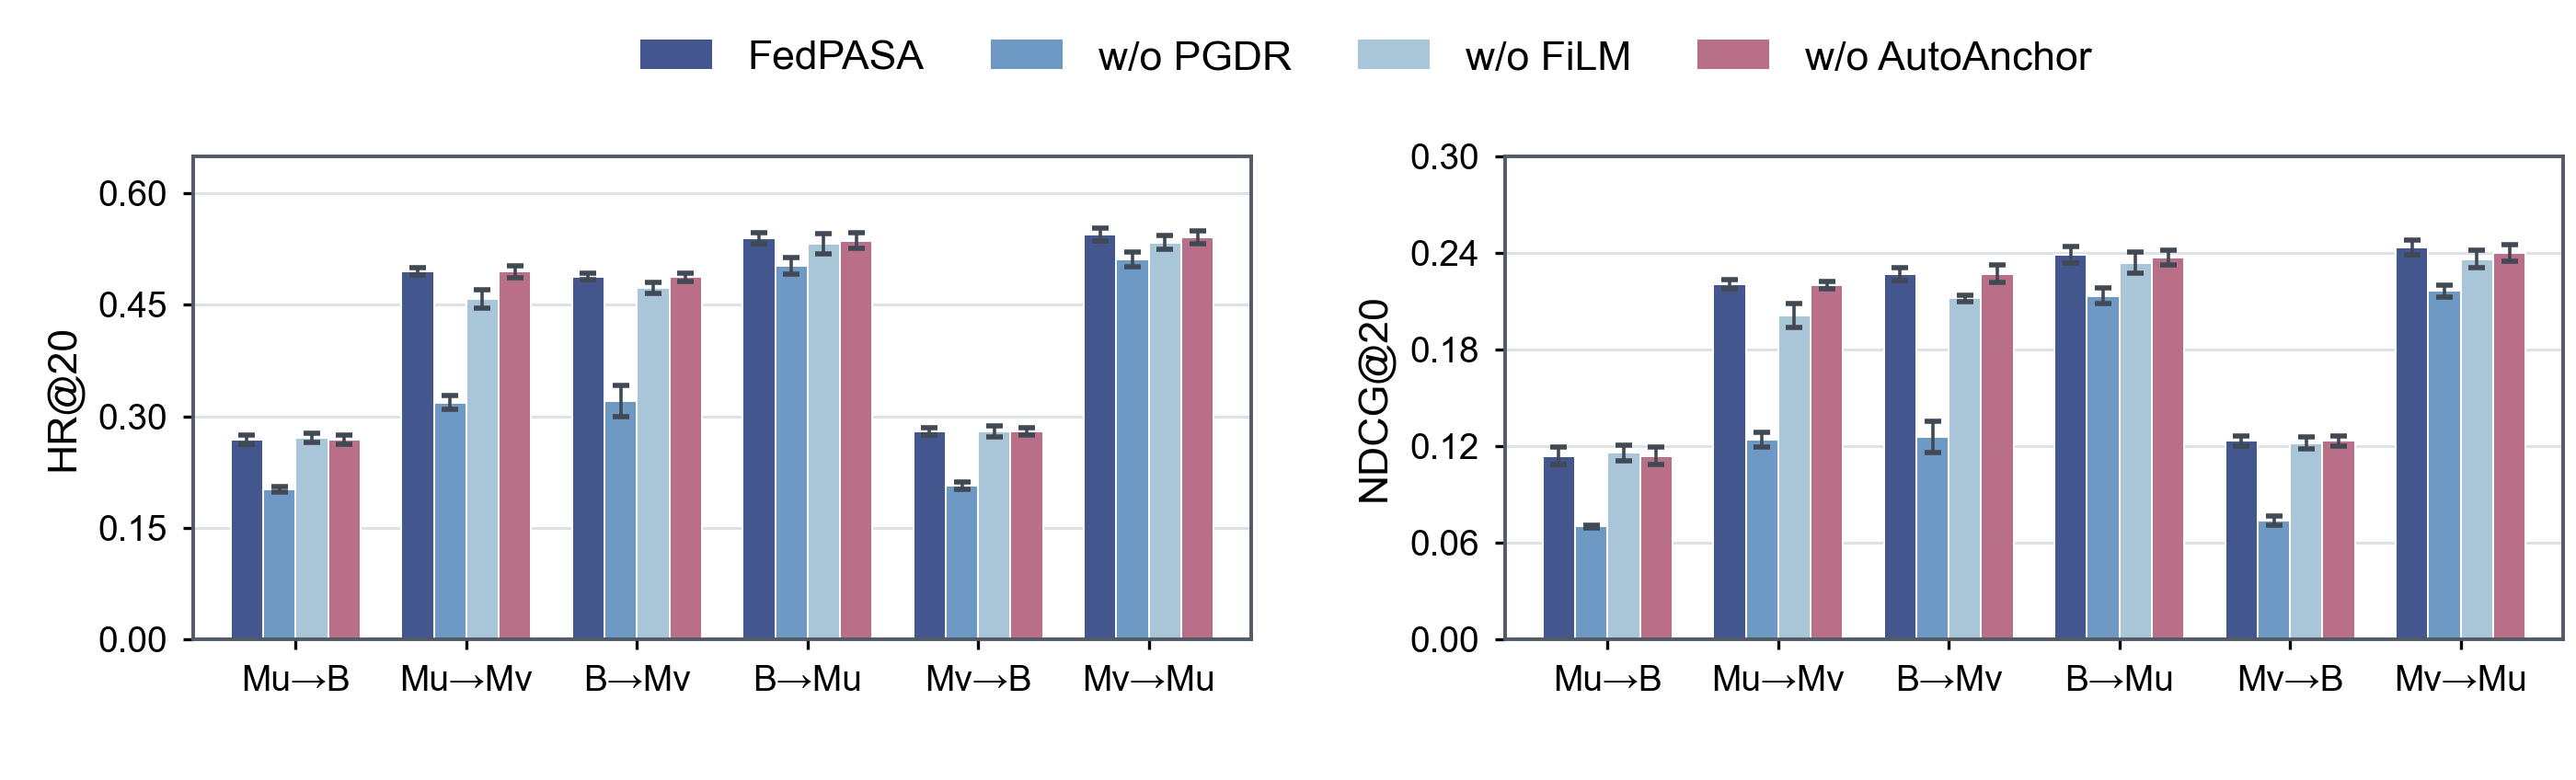
\includegraphics[width=\textwidth]{figures/component_ablation_selected.png}
\caption{Component ablations under 99-negative ranking before personalization (five-seed means $\pm$ SD). Mu: Music; B: Books; Mv: Movies. PGDR contributes most; FiLM and AutoAnchor have target-dependent effects.}
\Description{Two grouped bar charts report HR at 20 and NDCG at 20 for FedPASA and variants without routing, client conditioning, or anchoring across six transfer directions.}
\label{fig:component-ablation}
\end{figure*}

\begin{figure}[t]
\centering
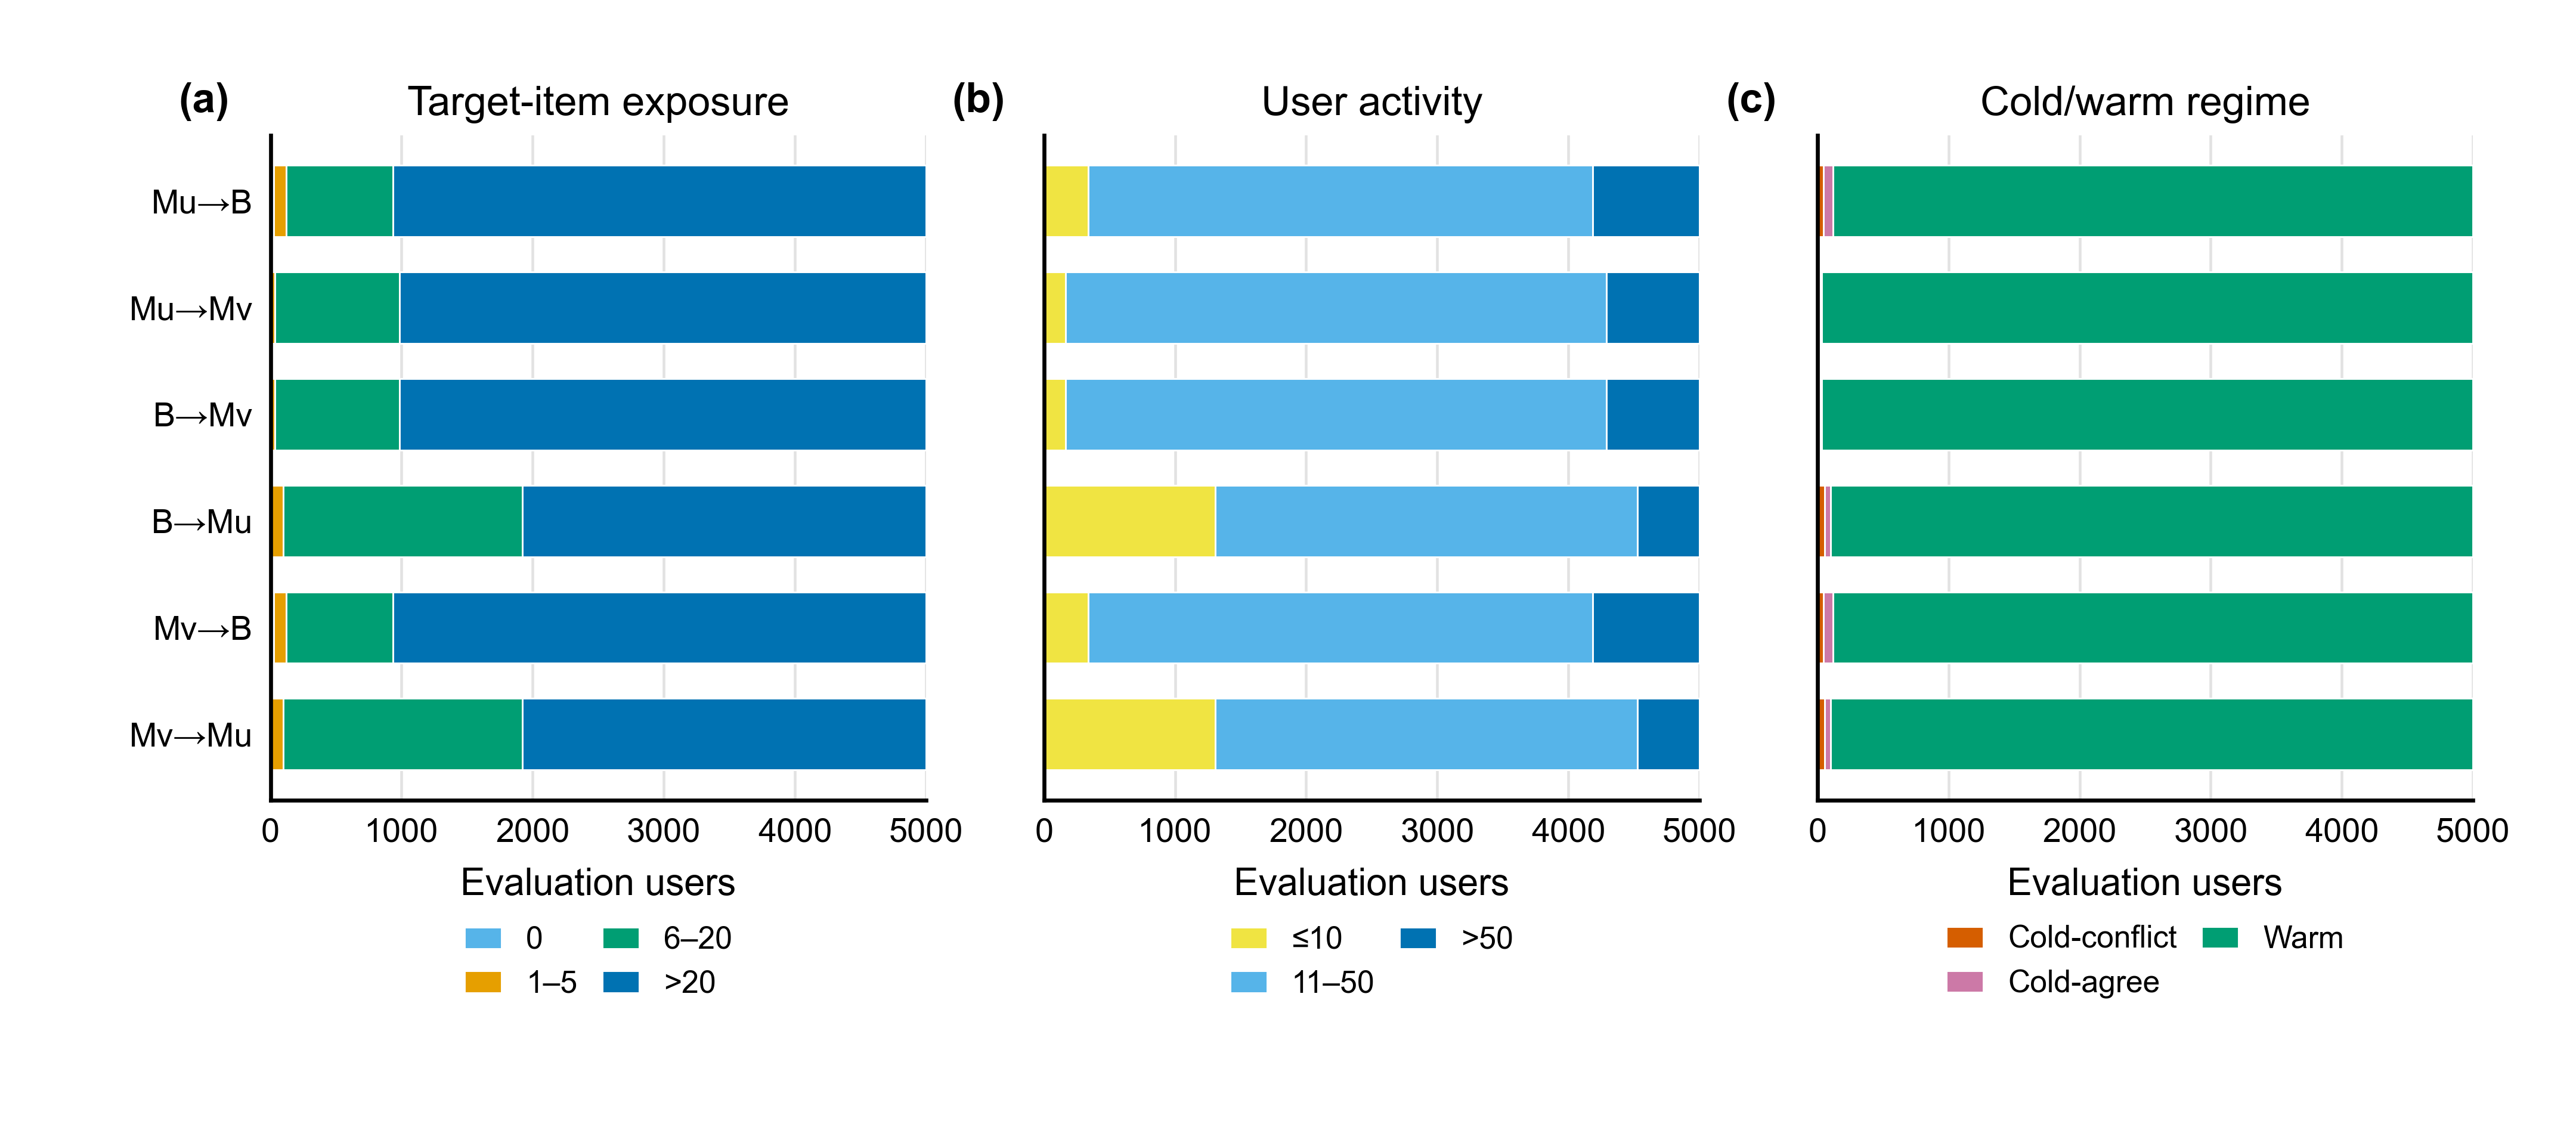
\includegraphics[width=\columnwidth]{figures/evaluation_slice_composition.png}
\caption{Evaluation-user composition: (a) target-item frequency, (b) user activity, and (c) cold/warm groups. Each transfer has 5,000 users. Mu/B/Mv: Music/Books/Movies.}
\Description{Three stacked bar charts show that evaluation users predominantly interact with frequent items, have moderate training activity, and belong to the warm group. The proportions vary across target catalogs.}
\label{fig:evaluation-slice-composition}
\end{figure}

\begin{table*}[t]
\centering\small
\caption{Joint frequency--exposure ablation before local personalization under full-catalog ranking. C/U: low-frequency items locally seen/unseen; W: frequency $>5$.}
\label{tab:joint}\label{tab:joint-ndcg}
\setlength{\tabcolsep}{6pt}
\renewcommand{\arraystretch}{1.12}
\begin{tabular*}{\textwidth}{@{\extracolsep{\fill}}l|rr|rr|rr@{}}
\toprule
\textbf{Model} & \multicolumn{2}{c|}{\textbf{C: low-frequency / seen}} & \multicolumn{2}{c|}{\textbf{U: low-frequency / unseen}} & \multicolumn{2}{c}{\textbf{W: frequency $>5$}} \\
 & HR@20 & NDCG@20 & HR@20 & NDCG@20 & HR@20 & NDCG@20 \\
\midrule
\textbf{FedPASA base} & \textbf{0.0160} & \textbf{0.0070} & \textbf{0.0347} & \textbf{0.0151} & \textbf{0.0102} & \textbf{0.0037} \\
% Lowest nonzero retained observations from outputs/www_v1/cross; pooled across six directions within each seed.
\textbf{w/o PGDR} & 0.0041 & 0.0010 & 0.0039 & 0.0013 & 0.0023 & 0.0007 \\
\textbf{w/o FiLM} & 0.0041 & 0.0018 & 0.0276 & 0.0123 & 0.0037 & 0.0014 \\
\textbf{w/o AutoAnchor} & 0.0082 & 0.0023 & 0.0144 & 0.0047 & 0.0039 & 0.0014 \\
\bottomrule
\end{tabular*}
\end{table*}



\begin{figure*}[t]
\centering
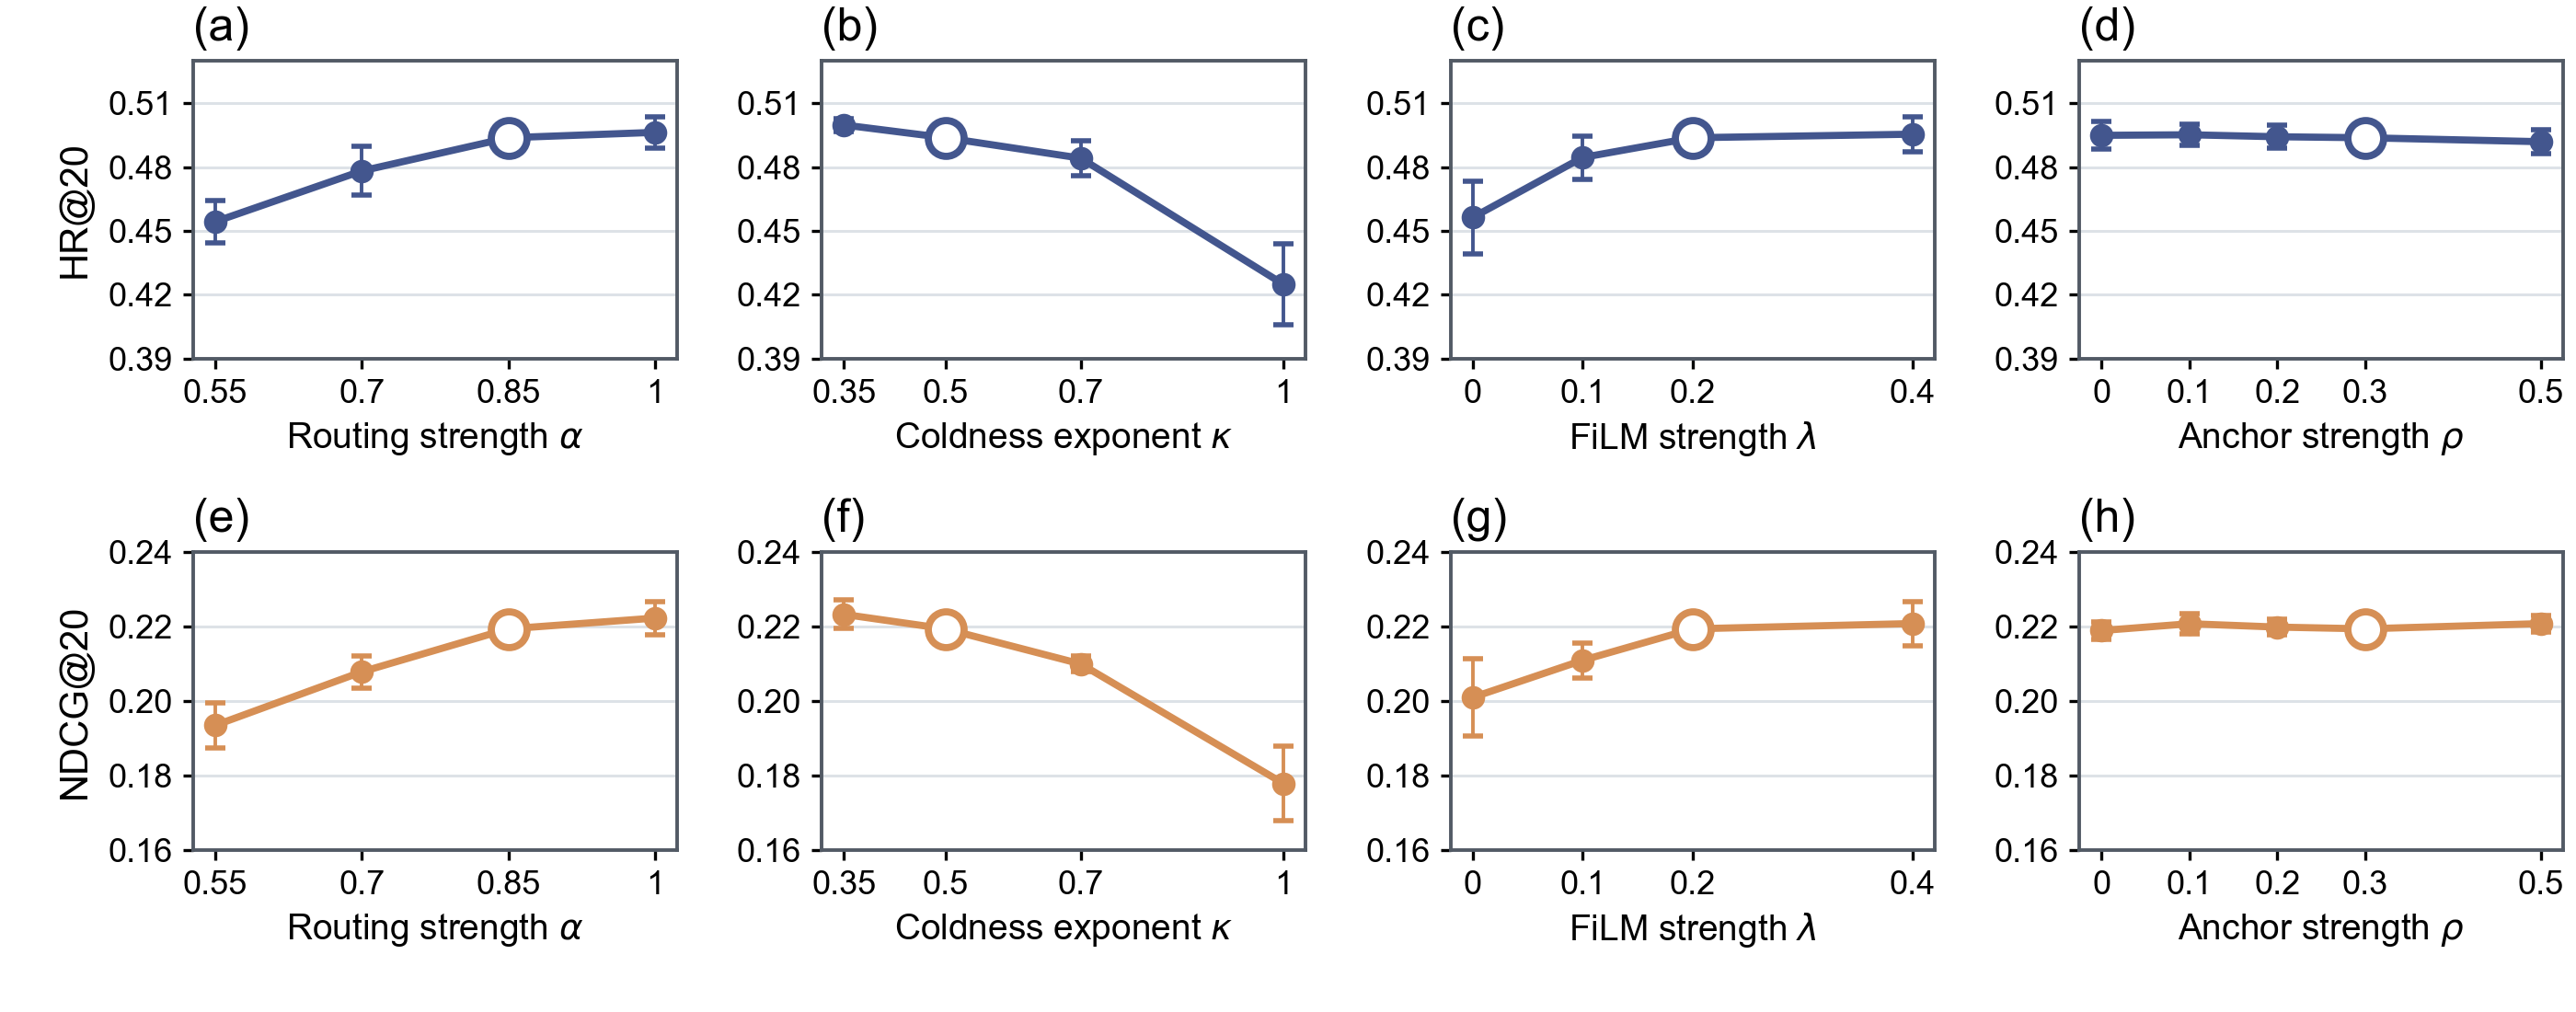
\includegraphics[width=\textwidth]{figures/sensitivity_selected.png}
\caption{Parameter sensitivity on Music$\to$Movies before personalization (99 negatives; three-seed means $\pm$ SD). Top: HR@20; bottom: NDCG@20. Each sweep varies one parameter. Open circles mark validation-selected defaults; vertical scales are shared within each row.}
\Description{Eight panels show the effects of routing strength, coldness exponent, FiLM strength, and anchor strength on HR and NDCG. Routing and coldness have larger effects than anchor strength.}
\label{fig:sensitivity}
\end{figure*}

\subsection{Experimental Settings}
\label{sec:exp-setup}
\subsubsection{Implementation Details}
We encode items with frozen DistilBERT-base-uncased representations ($d=768$) and use two-block residual adapters with bottleneck dimension 64 and dropout 0.1. All adapter methods are optimized with AdamW using a learning rate of $10^{-3}$ and weight decay of $10^{-4}$. Each BPR batch contains 32 positives and three negatives per positive. Cross-domain experiments use five clients and train for $12\times60$ rounds/local steps on Music and Movies and $8\times30$ on Books. FedMF uses 64-dimensional factors and $25\times80$ rounds/local steps. FedPASA sets $\mu=0$ during federation and performs $K_p=40$ personalization steps with $\mu_p=.15$. Validation on Music$\to$Movies selects $(\alpha,\kappa)=(.85,.5)$ and $(\lambda,\rho)=(.2,.3)$, which are fixed for all targets. We report HR and NDCG. Cross-domain evaluation uses a fixed 5,000-user subset with both 99-negative and full-catalog ranking; training and validation items are excluded from candidate sets. Common-backbone results are averaged over five runs. Additional baseline settings are given in Appendix~\ref{app:full}.

\subsubsection{Baselines}
We compare FedPASA with representative recent and classical federated recommendation baselines. \textbf{FeDecider}~\citep{he2026fedecider} uses LLM representations and client-specific directional weights to personalize LoRA aggregation. \textbf{TransFR}~\citep{zhang2026transfr} transfers a source-initialized language-model adapter and performs local personalization. \textbf{FFMSR}~\citep{lu2025ffmsr} transfers text-derived semantic representations in federated recommendation. \textbf{FedDCSR}~\citep{zhang2024feddcsr} disentangles shared and domain-specific factors for federated sequential recommendation. \textbf{FedMoE}~\citep{mei2024fedmoe} personalizes expert subsets through submodel search and modular aggregation. \textbf{FedAdam}~\citep{reddi2021adaptive} applies adaptive server-side optimization, while \textbf{FedProx}~\citep{li2020federated} adds a proximal term to constrain heterogeneous local updates. \textbf{pFedMe}~\citep{dinh2020personalized} couples personalized client parameters to a shared model through a proximal objective. \textbf{FedPer}~\citep{arivazhagan2019federated} combines a globally shared representation with client-specific personalization layers. \textbf{L2-SP}~\citep{li2018explicit} regularizes target parameters toward their source initialization. \textbf{FedAvg} learns one shared target adapter by averaging client updates, and \textbf{FedMF} keeps user factors local while aggregating item factors on the server. In the common-backbone comparison, all methods use the same frozen DistilBERT item features~\citep{sanh2019distilbert}, user partitions, and data splits; other baselines are evaluated with their corresponding datasets and ranking cutoffs.

\subsection{Main Results and Discussion (RQ1)}
\label{sec:exp-main}








\noindent\textit{Evidence-dependent adaptation improves transfer across disjoint catalogs.}
FedPASA leads both sampled-ranking metrics on all six transfers (Tables~\ref{tab:cross_main} and~\ref{tab:cross_main_remaining}), with a mean HR improvement of 14.2\% over FeDecider. The margins vary by target: gains are larger for Books and Movies, whereas the baselines are already competitive on Music. Frozen text features provide a shared semantic space, but do not determine how uneven target supervision should update that space. Frequency-dependent paths offer a plausible explanation for the additional gains; the ablations below isolate the contribution of each component.

\noindent\textit{The advantage extends beyond sampled candidates.}
FedPASA also leads the full-catalog comparison (Table~\ref{tab:full-directions}). The lower absolute accuracy is expected when many more items compete for the same top-ranked positions. Retaining the advantage supports improved discrimination beyond the sampled negatives, although Books remains difficult. This motivates examining both component effects and the item groups contributing to aggregate accuracy.

\subsection{Ablation Study (RQ2)}
\label{sec:exp-ablation}





Figure~\ref{fig:component-ablation} compares FedPASA with variants that remove one component at a time. All variants are evaluated before local personalization to isolate the adaptation modules; Tables~\ref{tab:cross_main} and~\ref{tab:cross_main_remaining} report the final personalized model. Error bars show variation across five seeds.

\noindent\textbf{(1) w/o PGDR.}
Using $h_i=A_h(x_i)$ removes frequency-dependent routing; both metrics decrease on every transfer. The equal-capacity controls retain both paths and the parameter count: constant routing removes item dependence, while shuffling breaks the frequency--weight correspondence. PGDR outperforms both controls, supporting frequency-dependent allocation of adaptation capacity (Table~\ref{tab:ablation}).

\noindent\textbf{(2) w/o FiLM.}
Setting $\lambda=0$ yields $m_{c,i}=h_i$ and removes client-dependent modulation. Average accuracy decreases, with clearer gains on Movies and Music and near-tied results on Books. Client conditioning thus complements routing, with a target-dependent contribution.

\noindent\textbf{(3) w/o AutoAnchor.}
Setting $\rho_{\mathrm{eff}}=0$ removes the frozen-prior contribution in Eq.~\eqref{eq:anchor}. Its average effect is smaller than that of routing or conditioning: Books results are identical because the catalog gate disables anchoring, while Music and Movies show modest changes. Representation drift is examined separately below.

\subsection{Evidence Mechanism Analysis (RQ3)}
\label{sec:exp-buckets}







Table~\ref{tab:joint} compares the component ablations across item groups defined jointly by frequency and local exposure. Each removal lowers both ranking metrics relative to FedPASA base, including for locally seen and locally unseen low-frequency items.

\noindent\textit{Group improvements and aggregate gains are distinct.}
Figure~\ref{fig:evaluation-slice-composition} shows that frequent items and warm cases dominate evaluation, while user activity and exposure vary across target catalogs. Consequently, aggregate metrics weight the groups unequally: strong relative gains in a small low-frequency group need not dominate overall accuracy. The finer slices in Table~\ref{tab:buckets} show that higher-frequency items contribute most of the full-ranking gain over FedAvg. Similar source-free and source-initialized averages (Table~\ref{tab:ablation}) further point to target-side adaptation as the main explanation.

\subsubsection{AutoAnchor and representation drift}
\label{sec:exp-anchor}\label{sec:exp-drift}
Preservation is measured separately from ranking through cosine distance:
\begin{equation}
D=\frac{1}{|\mathcal C||\mathcal I|}\sum_{c\in\mathcal C}\sum_{i\in\mathcal I}
\big(1-\cos(z^{\mathrm{anchor}}_{c,i},x_i)\big).
\end{equation}
Anchoring slightly reduces cold-item distance but increases the all-item average after training (Table~\ref{tab:drift}). Although Eq.~\eqref{eq:anchor} moves a fixed representation toward its prior before normalization, training changes the representation itself. The observed drift and ranking effects therefore depend on the item group and optimization outcome.

\subsection{Generalization and Robustness (RQ4)}
\label{sec:exp-robust}\label{sec:exp-noniid}







\noindent\textit{FedPASA remains effective under heterogeneous conditions.}
FedPASA exceeds TransFR in both metrics under all three non-IID Music$\to$Movies partitions (Table~\ref{tab:external-conditions}). More concentrated activity makes prediction harder, but the advantage persists. The table also examines client counts, fixed computation, partial participation, and update noise.

\noindent\textit{The gains are not tied to one feature encoder.}
The results extend to all evaluated directions with LLaMA features (Table~\ref{tab:external-conditions}), supporting semantic adaptation beyond a particular encoder.

\subsubsection{Sensitivity and statistical analysis}
\label{sec:exp-sens}\label{sec:exp-variability}







Figure~\ref{fig:sensitivity} separates the four adaptation controls. Increasing routing strength $\alpha$ improves both metrics over the tested range, whereas increasing coldness exponent $\kappa$ reduces them. FiLM gains largely saturate near $\lambda=.2$. The flatter response to $\rho$ is consistent with the catalog gate attenuating anchoring on this target. Open circles indicate defaults selected on validation data, not maxima of the plotted test curves. Table~\ref{tab:sensitivity-values} gives the numerical values.

The positive confidence interval for paired HR improvements over the learned-gate baseline supports a repeatable aggregate advantage; Tables~\ref{tab:seed-hr} and~\ref{tab:seed-ndcg} report variability.
